\chapter{Grundlagen}
\label{ch:Grundlagen2}

Dieses Kapitel beschreibt die grundlegenden Konzepte, die für das weitere Verständnis dieser Arbeit erforderlich sind. Abschnitt \ref{sec:Decision_Management2} behandelt Decision Mangement und gibt Aufschluss darüber, wie Entscheidungen automatisiert und verwaltet werden. In Abschnitt  \ref{sec:Machine_Learning2} folgt eine Einführung in das Machine Learning. Abschließend nennt Abschnitt \ref{sec:Technologien2} einsetzbare Lösungen zur Umsetzung der genannten Konzepte. 

\section{Decision Management}
\label{sec:Decision_Management2}

\emph{Decision Management} (DM) adressiert die Verwaltung von automatisierten Entscheidungen, über den kompletten Lebenszyklus von Entscheidungen hinweg. Dieser beinhaltet die Modellierung, Ausführung, Überwachung und die Optimierung, mit dem Ziel, fachliche Entscheidungen zu verbessern, indem der Lebenszyklus kontinuierlich durchlaufen wird. Abbildung \ref{fig:lifecycle} zeigt die einzelnen Phasen des Lebenszyklus.

\begin{figure}[ht]
\centering
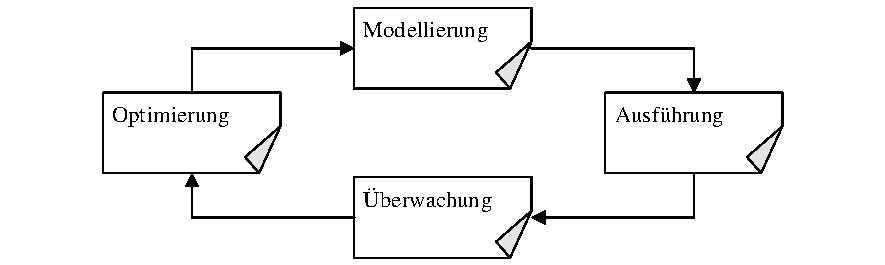
\includegraphics{images/lifecycle.pdf}
\caption{Der Lebenszyklus von automatisierten Entscheidungen.}
\label{fig:lifecycle}
\end{figure}

\textbf{Modellierung}. Zur Modellierung von Entscheidungen wurde 2015 der Standard Decison Model and Notation (DMN) von der Objekt Management Group veröffentlicht \cite[vgl. S. 7 ff.]{OM16}. Rücker nennt die Schaffung eines Notationsstandards für Entscheidungen, der für Fach- und IT-Anwender gleichermaßen verständlich ist, als übergeordnetes Ziel von DMN \cite[vgl. S. 40]{BR16}.  Die offizielle DMN-Spezifikation nennt die Erfüllung der folgenden drei Anforderungen als Ziel von DMN \cite[vgl. S. 18 ff.]{OM16}: 

\begin{enumerate*}
\item Modellierung von Entscheidungen, die von Menschen getroffen werden
\item Modellierung von Entscheidungen, die automatisiert getroffen werden 
\item Implementierung von automatisierten Entscheidungen    
\end{enumerate*}

Zur Umsetzung der genannten Anforderungen definiert DMN zwei verschiedene Ebenen: Die Entscheidungsanforderungsebene (deskriptiv) und die Entscheidungslogikebene (präskriptiv), beide zusammen bilden das \emph{Decision Model}. Auf der Entscheidungsanforderungsebene werden die Anforderungen, die eine Entscheidung benötigt, in einem Decision Requirements Diagrams (DRD) modelliert. Ein DRD besteht aus Entscheidungen, Input-Daten, Business Knowledge Models und Knowledge Sources. Abbildung \ref{fig:drd} \cite[vgl. S. 21]{OM16} zeigt die genannten Elemente eines beispielhaften DRD und deren Notation.     

\begin{figure}[ht]
\centering
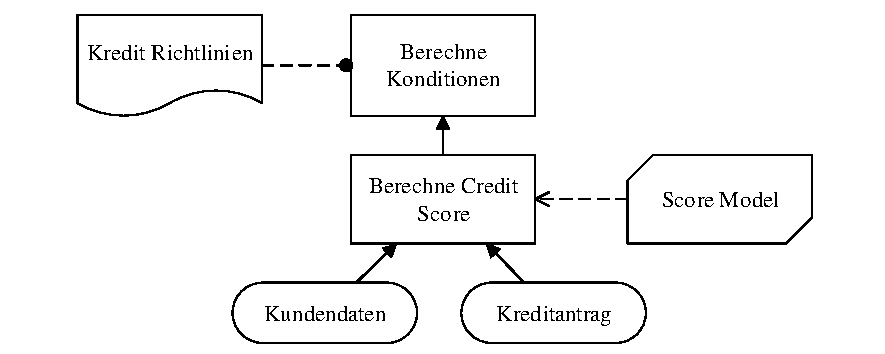
\includegraphics{images/drd.pdf}
\caption{Ein beispielhaftes DRD.}
\label{fig:drd}
\end{figure}

\begin{itemize*}

\item Ein Input-Data-Element beschreibt Informationen, die als Eingabe für eine oder mehrere Entscheidungen dient \cite[vgl. S. 30]{OM16}. Abbildung \ref{fig:drd} zeigt die beiden Input-Daten-Elemente Kundendaten und Kreditantrag. 

\item Ein Business Knowledge Model beschreibt eine Funktion die Fachwissen kapselt, beispielsweise als Geschäftsregel, Entscheidungstabelle oder als analytisches Model \cite[vgl. S. 30]{OM16}. In Abbildung \ref{fig:drd} kapselt das Score Model das Fachwissen zur Berechnung des Credit Scores.

\item Ein Decision-Element beschreibt eine Entscheidung. Sie bestimmt einen Output, anhand verschiedener Inputdaten, mithilfe von Entscheidungslogik \cite[vgl. S. 20]{OM16}. In Abbildung \ref{fig:drd} wird der Credit Score mittels der Inputdaten Kundendaten und Kreditantrag berechnet. Anschließend wird der Credit Score an die darüber liegende Entscheidung, zur Berechnung der Konditionen, weitergegeben.  

\item Eine Knowledge-Source beschreibt die Quelle einer Entscheidung oder eines Business Knowledge Models. Das kann beispielsweise ein Dokument oder auch ein Fach-Experte sein \cite[vgl. S. 18]{OM16}. Im vorliegenden Beispiel werden die Konditionen des Kredites durch die Vorgaben der Kredit Richtlinien berechnet.

\end{itemize*}

Nun gilt es sich der Entscheidungslogik-Ebene zu widmen, die insbesondere für die automatisierte Ausführung von Entscheidungen essentiell ist \cite[vgl. S. 18]{OM16}. DMN erlaubt den Import von existierenden Entscheidungslogik-Standards. Der wohl wichtigste Entscheidungslogik-Standard im Umfeld von DMN ist die Entscheidungstabelle. Taylor definiert Entscheidungstabellen als: ''a look-up table where each cell represents an executable business rule. The conditions of the rule are columns or rows in the decision table and the intersection of the rows and columns shows the consequence of the rule'' \cite[S. 132]{JT11}. Abbildung \ref{fig:decisiontable} zeigt eine Entscheidungstabelle zur Bestimmung des Zinses anhand eines Credit Scores. Wäre der Credit Score beispielsweise 632, würde die erste Zeile der Entscheidungstabelle zutreffen und der Zins 6 \%  betragen.

\begin{figure}[ht]
\centering
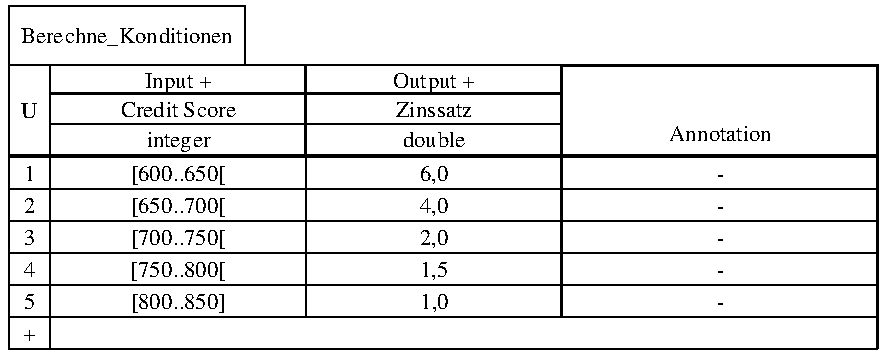
\includegraphics{images/decisiontable.pdf}
\caption{Beispiel einer Entscheidungstabelle zur Berechnung des Zinssatzes.}
\label{fig:decisiontable}
\end{figure} 

\textbf{Ausführung}. Um Decision Models ausführen zu können, müssen diese in einem geeigneten DMN-Tool modelliert werden. Zur vollständigen Automatisierung der Entscheidungen, muss die Entscheidungslogik in der Lage sein, für jeden möglichen Satz von Input-Daten einen
Entscheidungsausgang bestimmen zu können. Um eine effiziente Ausführung zu ermöglichen wird eine Decision Engine benötigt, die es erlaubt Entscheidungen in einer produktiven Einsatzumgebung auszuführen. ''Eine Decision Engine ist ein Stück Software, das eine zustandslose Schnittstelle bereitstellt, um Entscheidungen auf Basis der in DMN definierten Entscheidungslogik zu fällen'' \cite[S. 41]{BR16}. Nach der Inbetriebnahme der Decision Engine bedürfen die getroffenen Entscheidungen der Überwachung, um sicherzustellen, dass Entscheidungen so getroffen werden, dass deren Konsequenzen bestmöglich zur Erreichung der betriebswirtschaftlichen Ziele beitragen. 

\textbf{Überwachung}. Taylor nennt vier Faktoren, die kontrolliert werden sollen und dazu führen, dass Entscheidungen verbessert werden müssen \cite[vgl. S. 158]{JT11}:

\begin{enumerate*}
\item Änderungen an wirtschaftlichen Zielsetzungen
\item Neue Regularien oder Richtlinien
\item Änderungen an zugrundeliegenden Datenschemata  
\item Gesamt Performance der Entscheidungen\end{enumerate*}   

Auf die ersten drei Faktoren muss bei deren Eintritt reagiert werden, wohingegen der vierte Faktor einer ständigen Untersuchung bedarf. Proaktive Änderungen an Entscheidungslogiken bieten Möglichkeiten, die Effektivität unserer Entscheidungen zu steigern, um somit den wirtschaftlichen Zielsetzungen näher zukommen. Wie effektiv oder gut eine Entscheidung ist definiert Taylor wie folgt: ''The goals and key performance indicators or metrics of your business set a context that defines what a good or an effective decision looks like. The data you have collected over time gives you insight into what works and what doesn't, which is reflected in your current decision-making approach.'' \cite[vgl. S. 159]{JT11}. Die Analyse der Daten vergangener Entscheidungen ist somit unerlässlich, um proaktiv Entscheidungslogiken zu verbessern. Um eine effektive Überwachung und Verbesserung zu ermöglichen, müssen umfangreiche Datenmengen über die Effektivität von Entscheidungen gesammelt werden. Dazu zählen \cite[vgl. S. 164]{JT11}:

\begin{itemize*}
\item Ausführungs-Daten: Hierzu zählen alle Daten die während der Ausführung einer Entscheidung erhoben werden können. Beispielsweise IDs, Zeitstempel, Eingabe-Daten, Ausgabedaten, die Quelle des Aufrufs, oder kontextbezogene Daten die während der Ausführung generiert wurden.   
\item Antwort-Daten: Meistens ergibt sich aus einer Entscheidung heraus eine Konsequenz für den Empfänger der Entscheidung. Um nochmals das Beispiel der Online-Kredit-Bewerbung aufzugreifen, nachdem der Kreditantrag evaluiert und das Ergebnis zurückgeliefert wurde, kann die Reaktion des Empfängers gespeichert werden. Der Empfänger kann das zurückgelieferte Kreditangebot ablehnen, zustimmen, mehr Informationen verlangen oder für später abspeichern. Gelingt es die Reaktion des Empfängers mit der Entscheidung zur späteren Analyse abzuspeichern, können daraus wertvolle Rückschlüsse über die Effektivität der Entscheidung gewonnen werden.     
\item Andere Unternehmens-Daten: Neben den Daten die direkt oder indirekt durch die Entscheidung und ihre Konsequenz entstehen, macht es Sinn weitere Unternehmensdaten an vergangene Entscheidungen zuknüpfen, die später in unserer Überwachungsumgebung zu sehen sein sollen. Bei einer Entscheidung zur Berechnung der Bonität beispielsweise würde die Information, ob es zu Zahlungsausfällen kam, verknüpft mit dem entsprechenden Entscheidungsdatensatz erlauben, direkte Aussagen über die Effektivität der Entscheidungslogik zu treffen.       
\end{itemize*}         

Eine entsprechende Überwachungsumgebung müsste all diese Daten sammeln und aufbereiten, so dass der komplette Entscheidungsfindungsprozess und die daraus resultierenden Ereignisse im Nachhinein noch nachvollzogen werden können.

\textbf{Optimierung}. Um bestehende Entscheidungen optimieren zu können, bedarf es einer Simulations-Umgebung in der verschiedene Ansätze gegeneinander getestet werden können. Ein mögliches Szenario könnte so aussehen, dass man die Entscheidungslogik im Produktiveinsatz, in einem A/B Test gegen eine neue Entscheidungslogik testet. Testet man fortlaufend parallel verschiedene Ansätze kann man erkennen, welche sich langfristig am effektivsten auf wirtschaftliche Zielsetzungen auswirken \cite[vgl. S. 173]{JT11}. \emph{Predictive Analytics} eignen sich um neue Entscheidungslogiken zu entwickeln. Predictive Analytics bezeichnet \cite[vgl. S. 5]{BG15} das Verwenden von Verfahren aus der Statistik, sowie dem Machine Learning um vorherzusehen, mit welcher Wahrscheinlichkeit ein ungewisses Ereignis eintritt.   
  
\section{Machine Learning}
\label{sec:Machine_Learning2}

\emph{Machine Learning} (ML) ist eines der zentralen Themengebiete innerhalb der  \emph{Künstlichen Intelligenz} (KI) \cite[vgl. S. 2082]{JW12} und beschreibt das Forschungsgebiet das Computer befähigt zu lernen, ohne explizit dafür programmiert worden zu sein \cite[vgl. S. 1]{AM14}. Lernen im Kontext von ML definieren Mitchell et al. als: ''A computer program is said to learn from experience E with respect to some class of tasks T and performance measure P if its performance at tasks in T, as measured by P, improves with experience E'' \cite{MT97}. Soll beispielsweise ein Programm implementiert werden, das aufgrund vergangener Banktransaktionen (Experience E) lernen soll wie man betrügerische Banktransaktionen erkennt (Task T), benötigen die Datensätze der Banktransaktionen ein weiteres Attribut, das angibt ob sich die Transaktion als Betrug, oder echt erwiesen hat (Performance P).        Der Zusammenhang zwischen Ursache und Wirkung soll mit Hilfe eines Models beschrieben werden. Das Modell soll aus den Erfahrungen der Vergangenheit auf Ergebnisse in der Zukunft schließen können. Dabei wird versucht Eingabe- auf Ausgabewerte abzubilden, so dass die Differenz zwischen dem vorhergesagt Wert und dem realen Wert möglichst klein ist \cite[vgl. S. 68]{EM17}. 

Abhängig von der zugrundeliegenden Problemstellung, wird zwischen verschiedenen Lernprinzipien unterschieden:    

\begin{enumerate*}
\item Supervised Learning: 
\item Unsupervised Learning: 
\item Reinforcement learning:
\end{enumerate*}    

..................................................................
..................................................................

- Was ist Machine Learning

- Arten von Algorithmen 

- Neuronale Netze 

- Übergang: Es gibt viele verschiedene Algorithmen etc. allerdings macht es keinen Sinn mehr diese selbst zu implementieren -> Verwendung von Frameworks und somit überleiten auf nächste Kapitel

\section{Technologien}
\label{sec:Technologien2}

- Verwendung von Frameworks erforderlich um Effizient zu sein.

- Rad nicht neu erfinden evtl. Studie zur Verwendung von Frameworks.

\subsection{Decision Management}
\label{subsec:Decision_Management2}

- ACTICO 
- SAS
- FICO 
- Signavio
- Camunda

\subsection{Machine Learning}
\label{subsec:Machine_Learning2}

- Neuroph
- Aerosolve 
- Deeplearning4j
- Appache Spark

DELETED:

Decision Management Systeme (DMS) wurden entwickelt, um diesem Bedürfnis nachzukommen, mit dem Anspruch gleichzeitig agil, analytisch und adaptiv zu sein \cite[vgl. S. 1]{JT12}. \textit{Agil}, damit DMS anpassungsfähig auf sich ständig ändernde Regulationen und Marktbedingungen bleibt \cite[vgl. S. 4]{JT11}. \textit{Analytisch}, indem Entscheidungen modelliert werden, die mit Hilfe von Analyse- und Visualisierungstools optimiert werden, damit Entscheidungen analytisch getroffen werden \cite[vgl. S. 8]{JT11}. \textit{Adaptiv}, indem DMS es ermöglichen, neue Ansätze zu erlernen und zu testen, um Geschäftsziele durch neue Herangehensweisen zu erreichen \cite[vgl. S. 15]{JT11}. Taylor behauptet \cite[vgl. S. 1]{JT12}, dass traditionelle Informationssysteme zu unflexibel sind, um den Anforderungen von Verbrauchern, Aufsichtsbehörden und denen des Marktes nachzukommen. Aus diesem Grund werden die zu verbessernde Entscheidungen in dieser Arbeit in einem DMS modelliert und ausgeführt. 

Wichtig zu beachten ist, dass die Verwendung von BKM zur Kapselung von Fachwissen nicht zwingend notwendig ist. Das Kapseln von Fachwissen kann je nach Modellier-Still über ein BKM oder direkt in die Entscheidung hinein erfolgen. Entscheidungen dürfen somit mit keinem, oder beliebig vielen BKM verbunden werden \cite[vgl. S. 60]{OM16}.

Bei der Implementierung eines Decision Management Systems ist der wichtigste Schritt \cite[vgl. S. 115]{JT11}, dass ein Decision Service als IT-Komponente gebaut wird, der einerseits die gewünschte Entscheidung liefert und andererseits in die bestehenden Systemlandschaften integriert werden kann. Der Decision Service sollte also stets dem Konzept der Service-Oriented-Architecture (SOA) gerecht werden. Allerdings sollte nicht jede Entscheidung innerhalb eines DRDs als DS implementiert werden, sondern nur High-Level Entscheidungen die auch außerhalb des DMS von anderen Prozessen, Events oder Systemen benötigt werden \cite[vgl. S. 116]{JT11}. Eine konkrete Implementierung könnte so aussehen, dass ein DRD sowie die darunter liegende Entscheidungslogik mittels eines DMN-Tools modelliert wird. DMN-Tools bieten Programmierschnittstellen, über die die Entscheidungen angesteuert werden können. Um die Kommunikation mit anderen Systemen zu ermöglichen, müsste eine Decision-Engine \cite[vgl. S. 41]{BR16} entwickelt werden, die einerseits die Entscheidung anstößt und darüber hinaus einen Webservice definiert, über den Input-Daten und Entscheidungsausgang kommuniziert werden können. Abbildung zeigt alle Komponenten die zur Implementierung benötigt werden sowie deren Zusammenspiel.


Nach der theoretischen Beschreibung von DM und ML, werden einsetzbare Lösungen identifiziert,  die zur Implementierung des Prototypen verwendet werden können. Darüber hinaus wird dieses Kapitel darüber Aufschluss geben, wie diese zwei Grundlagenthemen zusammenhängen (siehe Abbildung \ref{fig:Grundlagenpic}).     

\begin{figure}[ht]
\centering
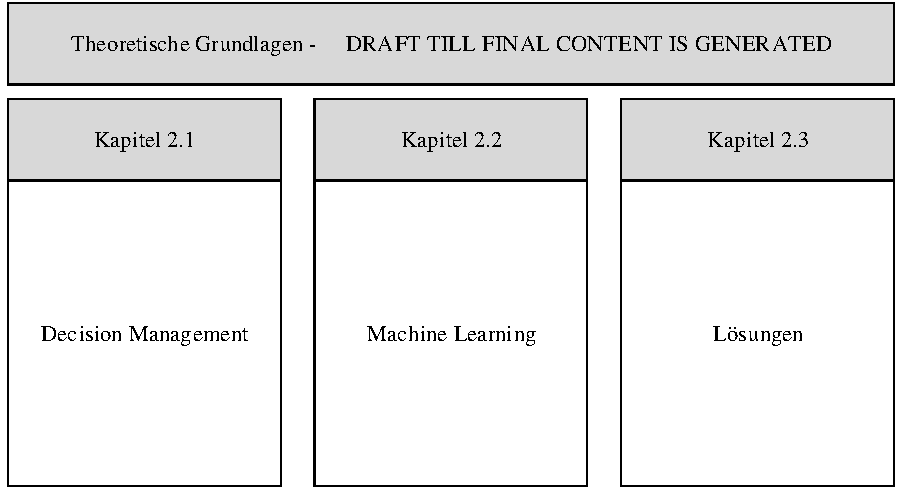
\includegraphics{images/grundlagentheo.pdf}
\caption{Die theoretischen Grundlagen im Überblick}
\label{fig:Grundlagenpic}
\end{figure}

Die Einzelnen Kapitel im Detail erklären .... (Erst möglich nachdem Sie geschrieben wurden)

Zu Beginn dieses Kapitels wurden DMS drei Kerneigenschaften zugesprochen, die maßgeblich für einen erfolgreichen Einsatz sind. Eine Eigenschaft war, dass Entscheidungslogiken unter Verwendung von Statistischen-Modellen optimiert werden. An dieser Stelle soll diese Arbeit untersuchen, ob Machine-Learning-Verfahren verwendet werden können um Entscheidungslogiken zu verbessern. Taylor behauptet Machine-Learning-Verfahren, zur Optimierung von Entscheidungslogik, können nur in den wenigen nachfolgenden Szenarien verwendet werden \cite[vgl. S. 179]{JT11}: 

\begin{enumerate*}
\item Wenn es innerhalb einer Organisation, keine Fachexperten für Analytics gibt 
\item Wenn sich Statistische-Modelle so oft ändern, dass nur ein automatisierter Ansatz in Frage kommt
\item Wenn die Genauigkeit des Statistischen-Modells keinen hohen Stellenwert besitzt
\item Wenn noch keine historischen Daten gesammelt wurden      
\end{enumerate*} 

Darüber hinaus behauptet Taylor \cite[vgl. S. 179]{JT11}, dass ML-Verfahren nicht in regulierten Industrien eingesetzt werden können, da sich ML-Modelle nicht erklären lassen, was ein Nachvollziehen einer Entscheidung im Nachhinein unmöglich macht. Diese Problemstellung soll im weiteren Verlauf dieser Arbeit kritisch hinterfragt werden. Zuvor werden jedoch  die Grundlagen von Machine Learning, in Kapitel \ref{sec:Machine_Learning2} erläutert.

Studien wie zeigen dass im Jahr 2016, 84 Prozent der Weltbevölkerung Zugang zu mobilen Breitband-Netzwerken haben. Regierungschefs der G20 Länder, haben sich darauf verständigt, dass die komplette Weltbevölkerung, bis zum Jahr 2025, Zugang zum Internet erhalten soll. Neben der wachsenden Anzahl an Teilnehmern im Internet, wächst auch die Anzahl an Maschinen die mit anderen Maschinen kommunizieren. Einhergehend mit den Teilnehmern im Internet, wächst auch die Anzahl an Diensten die online abgerufen werden können. Der rasante Wachstum der genannten beiden Faktoren resultiert in einem enormen anstieg des Datenvolumens. Studien haben ergeben , dass sich das weltweite Datenvolumen alle zwei Jahre verdoppelt.       

Studie 84% der Weltbevölkerung haben zugang zu einem 3G Breitband Zugang
http://www.itu.int/en/ITU-D/Statistics/Documents/facts/ICTFactsFigures2016.pdf 

Studie doppeltes Datenvolumen alle 2 Jahre:
https://www.emc.com/leadership/digital-universe/2014iview/executive-summary.htm

G20
https://www.heise.de/newsticker/meldung/G20-Laender-streben-Internet-fuer-alle-bis-zum-Jahr-2025-an-3678270.html

IOT:
http://www.gartner.com/newsroom/id/3165317

Big Data

Supervised 

Unsupervised

Neural Netwrork